\chapter{控制台应用程序设计}
\label{chp:Terminal-application-programming}

\section*{基本信息}
\sline
\begin{description}
\item[课程名称:] Java应用与开发
\item[授课教师:] 王晓东
\item[授课时间:] 第五周
\item[参考教材:] 本课程参考教材及资料如下:
  \begin{itemize}
  \item 陈国君主编,Java程序设计基础(第5版),清华大学出版社,2015.5
  \item Bruce Eckel, Thinking in Java (3rd)
  \end{itemize}
\end{description}

\section*{教学目标}

\sline

\begin{enumerate}
\item 了解计算机人机交互发展
\item 掌握控制台程序设计开发中命令行参数、系统属性、标准输入输出的概
  念和相关Java操作
\item 掌握Java文件操作的的常用方法
\item 了解注解类型
\item 学会Jar归档工具,包括通过命令行或IDE进行Java程序归档的方法
\end{enumerate}

\section*{授课方式}

\sline
\begin{description}
\item[理论课:] 多媒体教学、程序演示
\item[实验课:] 上机编程
\end{description}

\newpage
\section*{教学内容}
\sline

\section{从古老的计算机谈起}

\subsection{冯诺依曼机}

我们的计算机是台遵守存储程序原理的冯诺依曼机器,基本组成包括{\hei 运算
  器、控制器(合起来是CPU)、存储器、输入设备、输出设备}。你所面对的一
切SOC也好,单板电脑也好,都是高度集成在一起的冯诺依曼机。

\subsubsection{1950年代的IBM 1401}

\begin{figure}[htb]
\centering
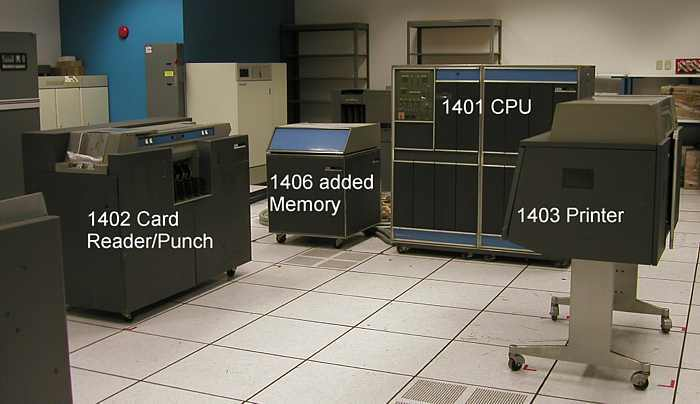
\includegraphics[width=0.6\textwidth]{images/Terminal-application-programming/fig-old-computer-01.jpg}
\caption{IBM 1401}
\label{fig:old-computer-01.jpg}
\end{figure}

\subsubsection{2010年代的树莓派开发板}

\begin{figure}[htb]
\centering
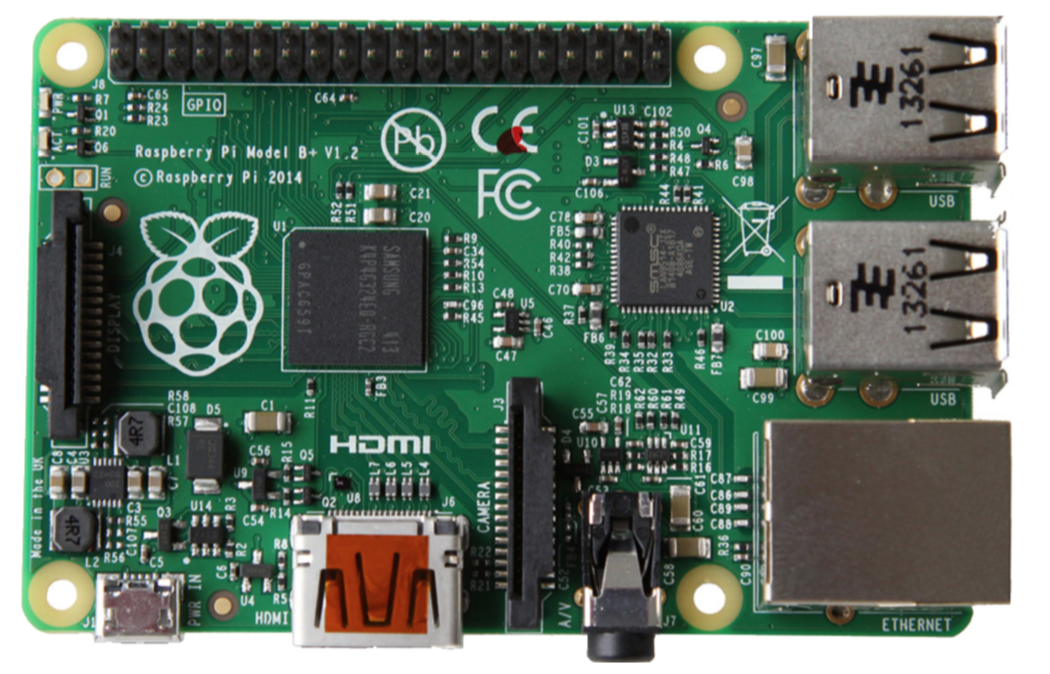
\includegraphics[width=0.5\textwidth]{images/Terminal-application-programming/fig-Raspberry-Pi-Board.png}
\caption{树莓派开发板}
\label{fig:Raspberry-Pi-Board}
\end{figure}


\subsection{人机交互}

\subsubsection{使用打孔卡片作为输入源,使用打印机作为输出设备}

一摞打孔卡片,就是一个“文件”。它可以是一段程序,也可以是一段程序需要使用的数据。

\begin{figure}[htb]
\centering
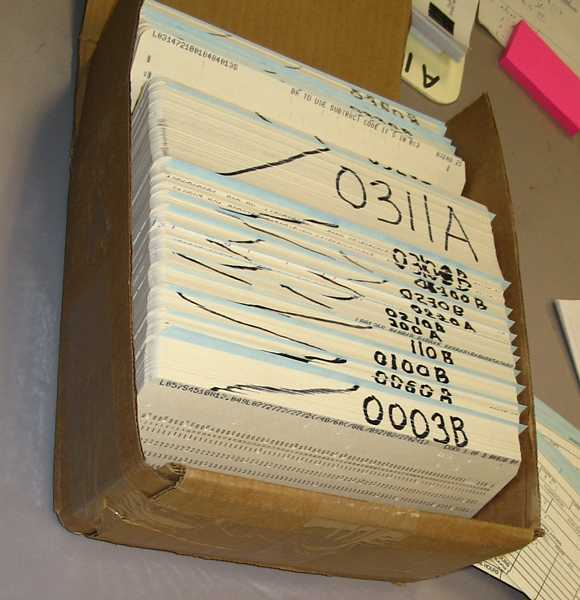
\includegraphics[width=0.5\textwidth]{images/Terminal-application-programming/fig-old-computer-input.jpg}
\caption{打孔卡片}
\label{fig:old-computer-input}
\end{figure}

\subsubsection{BASIC语言解释器}

纸带在70年代还很流行,当年比尔盖茨的BASIC语言解释器,就是存在纸带上的,现在已经成文物了。

\begin{figure}[htb]
\centering
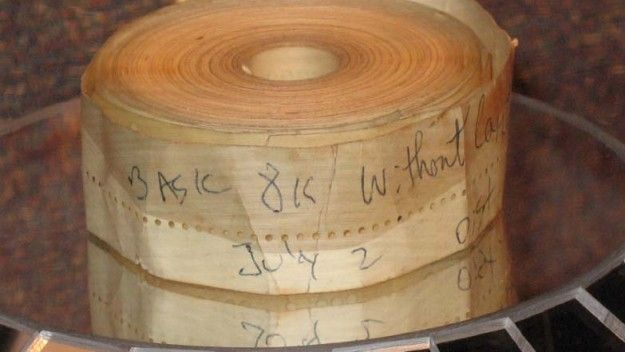
\includegraphics[width=0.6\textwidth]{images/Terminal-application-programming/fig-basic-lang-punch-tape.jpg}
\caption{打孔卡片}
\label{fig:basic-lang-punch-tape}
\end{figure}

\subsubsection{使用键盘作为输入设备,使用显示器作为输出设备}

\begin{figure}[htb]
  \begin{minipage}[t]{0.5\textwidth}
    \centering
    \fbox{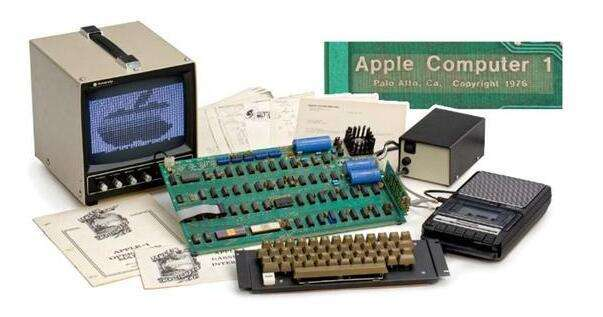
\includegraphics[width=.95\textwidth]{images/Terminal-application-programming/fig-apple-1-modules.jpg}}
    \caption{分立的Apple I}
    \label{fig:apple-1-modules}
  \end{minipage}
  \begin{minipage}[t]{0.5\textwidth}
    \centering
    \fbox{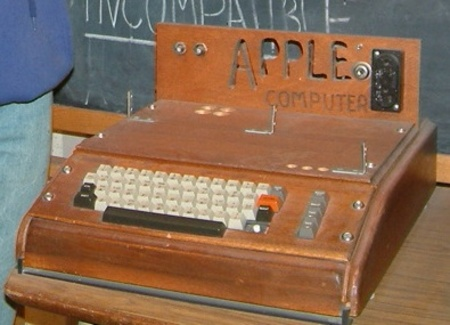
\includegraphics[width=.95\textwidth]{images/Terminal-application-programming/fig-apple-1.jpg}}
    \caption{Apple I}
    \label{fig:apple-1}
  \end{minipage}
\end{figure}

再厉害的科幻片导演,在飞船的人机交互界面表达上也未能超越同时代计算机的发展。

\begin{figure}[htb]
\centering
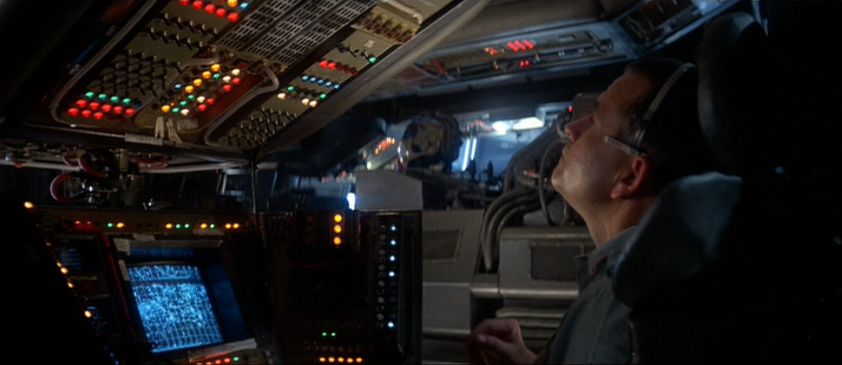
\includegraphics[width=\textwidth]{images/Terminal-application-programming/fig-Al012.png}
\caption{科幻定影中的计算机}
\label{fig:Al012}
\end{figure}

\section{命令行参数}

\subsection{命令行参数}

在启动时Java控制台应用程序,可以一次性地向程序中传递(零至多个)字符串参
数,这些参数被称为命令行参数。语法格式如下:

\begin{shCode}
  java <应用程序类名> [<命令行参数>]*
\end{shCode}

\notice{说明}

\begin{itemize}\kai
\item 命令行参数将被系统接收并静态初始化为一个一维的String数组对象,然后将之作为实参传给
  应用程序入口方法main()。
\item 命令行参数须使用空格符分隔,如果参数中包含空格符则必须使用双引号括起来。
\end{itemize}


\codeset{sample.commandline.CommandLineArgsSample.java}

Linux下运行程序方法如下:

\begin{shCode}
  > java CommandLineArgsSample Lisa "Billy" "Mr Brown"
\end{shCode}

Windows下运行程序方法如下:

\begin{shCode}
  C:\> java.exe CommandLineArgsSample Lisa "Billy" "Mr Brown" "a""b" 
\end{shCode}

输出结果为:

\begin{stdoutCode}
  Lisa
  Billy
  Mr Brown
\end{stdoutCode}


\subsection{可变参数方法}

\begin{itemize}
\item Java语言允许在定义方法时指定使用任意数量的参数,其格式是在参数
  类型后加“...”。
\item 可变长度参数必须放在参数列表的最后,一个方法最多只能包含一个可
  变长度参数。
\item 编译时,可变参数被当作{\Red\hei 一维数组处理}。
\end{itemize}

\begin{javaCode}
  public void myprint(String s, int i, Object... objs) { // 可变参数方法
    System.out.println(s.toUpperCase()); 
    System.out.println(100 * i);
    for(Object o: objs) { // 作为一维数组处理
      System.out.println(o); 
    }
  } 
\end{javaCode}


\section{系统属性}

\subsection{系统属性概述}

\begin{itemize}
\item 记录当前操作系统和JVM等相关的环境信息。
\item 以{\hei\Red 键值对}的形式存在,由{\hei\Red 属性名称、属性值}两部分组成。
\item 均为字符串形式。
\end{itemize}
  
系统属性的用途主要包括:

系统属性在URL网络编程、数据库编程和Java Mail邮件收发等编程中经常使用,
一般被用来设置代理服务器、指定数据库的驱动程序类等。

除了使用代码方法外,也可使用命令在运行程序时添加新的系统属性:
  
\begin{shCode}
  >java -Dmmmm=vvvv SystemPropertiesSample
\end{shCode}

\subsection{遍历、操作系统属性}

可以使用System.getProperties()获得一个封装了当前运行环境下所有系统属性
信息的Properties类(java.utils.Properties)的实例。

\codeset{sample.commandline.SystemPropertiesSample.java}

Properties类的可用方法包括:

\begin{description}
\item [\fbox{Enumeration propertyNames()}] 返回以Enumeration类型表示的所有可用系统属性的名称。
\item [\fbox{String getProperty(String key)}] 获得特定系统属性的属性值。
\item [\fbox{Object setProperty(string key, String value)}] 设置/添加单个系统属性信息。
\item [\fbox{void load(InputStream inStream)}] 
\item [\fbox{void store(OutputStream out, String header) }] 实现属性信息的导入/导出操作。
\end{description}

\section{标准输入/输出}

\subsection{标准输入/输出概述}

控制台程序的交互方式中:

\begin{itemize}
\item 用户使用键盘作为{\hei 标准输入设备}向程序输入数据
\item 程序利用计算机终端窗口作为{\hei 程序标准输出设备}显示输出数据
\end{itemize}

这种操作被称为{\hei 标准输入/输出(Standard Input/Output)}。

\subsection{标准输入/输出的分类}

java.lang.System类的三个静态类成员提供了有关标准输入/输出的IO操作功能。

\begin{description}\kai
\item [System.in] 从“标准输入”读入数据(java.io.InputStream类型)
\item [System.out] 向“标准输出”写出数据(java.io.PrintStream类型)
\item [System.err] 向“标准错误”写出数据(java.io.PrintStream类型)
\end{description}

PrintStream类的主要方法print()/println()方法被进行了多次重载
(boolean、char、int、long、float、double以及char[], Object和String)。

\subsection{读取控制台输入的传统方法}

\begin{javaCode}
  import java.io.InputStreamReader; 
  import java.io.BufferedReader; 
  import java.io.IOException;

  public class TestStandardInput {
    public static void main (String args[]) {
      String s;
      InputStreamReader isr = new InputStreamReader(System.in); 
      BufferedReader br = new BufferedReader(isr);
      try {
        s = br.readLine(); 
        while (!s.equals("")) {
          System.out.println("Read: " + s);
          s = br.readLine(); 
        }
        br.close();
      } catch (IOException e) {
        e.printStackTrace(); 
      }
    } 
  }  
\end{javaCode}

对上述程序的几点解释:

\begin{itemize}
\item System.in为InputStream类型对象,功能较弱,只能以字节为单位从预定
  义的标准输入(键盘)读取信息。
\item 程序并没有直接操作System.in对象进行读取操作,而是将其封装为一个功
  能稍强的InputStreamReader对象,以字符为单位读取信息。实际的过程
  为:{\kai InputStreamReader对象并没有直接读取键盘输入,而是多次调
    用System.in对象的读字节功能,再将所得字节转换为字符。}
\item InputStreamReader仍不能令人满意,再次封装,得到BufferedReader对
  象。后者提供了缓冲读取的功能,即多次调用InputStreamReader读字符操作,
  然后将所读取的多个字符积累起来组成字符串,其间以换行符为分隔,最终
  实现以行为单位读取字符串功能。
\item 当在键盘上空回车时,BufferedReader的readLine()方法接收到的不是
  空值null,而是一个长度为零的字符串"",其中包含0个字符但仍然是一
  个Java对象。
\end{itemize}

\section{文件操作}

\subsection{文件操作对象}

java.io包中定义与数据输入、输出功能有关的类,包括提供文件操作功能
的File类。我们可以使用以下构造方法创建File类对象:

\begin{itemize}
\item public File(String pathname)\\
  通过给定的路径/文件名字符串创建一个新File实例。
\item public File(String parent, String child)\\
  通过分别给定的parent路径名和child文件名(也可以是子路径名)或字符串来
  创建一个新File实例。
\end{itemize}

\subsection{使用File类}

\codeset{sample.commandline.FileOperationSample.java}

\subsection{File类的主要方法} 

\subsubsection{文件/目录名操作}

\begin{itemize}
\item String getName() 
\item String getPath() 
\item String getAbsolutePath() 
\item String getParent()
\end{itemize}

\subsubsection{设置和修改操作} 
    
\begin{itemize}
\item boolean delete() 
\item void deleteOnExit() 
\item boolean createNewFile() 
\item setReadOnly() 
\item boolean renameTo(File dest)
\end{itemize}

\subsubsection{测试操作} 

\begin{itemize}
\item boolean exists() 
\item boolean canWrite() 
\item boolean canRead() 
\item boolean isFile() 
\item boolean isDirectory() 
\item boolean isAbsolute()
\end{itemize}

\subsubsection{目录操作}

\begin{itemize}
\item boolean mkdir() 
\item String[] list() 
\item File[] listFiles()
\end{itemize}

\subsubsection{获取常规文件信息操作}

\begin{itemize}
\item long lastModified() 
\item long length()
\end{itemize}


\subsection{文件I/O有关读写类}

常见的文本文件I/O操作的类包括:
\begin{itemize}
\item java.io.FileReader类\\
  提供read()方法以字符为单位从文件中读入数据。
\item java.io.FileWrite类\\
  提供write()方法以字符为单位向文件写出数据。
\item java.io.BufferedReader类\\
  提供readLine()方法以行为单位读入一行字符。
\item java.io.PrintWriter类\\
  提供print()和println()方法以行为单位写出数据。
\end{itemize}


\subsection{读取文件内容}

\samp{ReadFileSample.java}

\begin{javaCode}
  import java.io.*;

  public class ReadFileSample {
    public static void main (String[] args) {
      String fname = "test.txt"; 
      File f = new File(fname);

      try {
        FileReader fr = new FileReader(f);  // 1
        BufferedReader br = new BufferedReader(fr); 
        String s = br.readLine();
        while (s != null) { // 2
          System.out.println("读入:" + s);
          s = br.readLine(); }
        br.close();
      } catch (FileNotFoundException e1) {
        System.err.println("File not found: " + fname); 
      } catch (IOException e2) {
        e2.printStackTrace(); 
      }
    } 
  }
\end{javaCode}

\notice{上述代码几点说明}

\begin{enumerate}
\item FileReader的构造方法被重载过,接受以字符串形式给出的文件名,上述代码等价于:
  \begin{javaCode}
    FileReader fr = new FileReader("test.txt");
  \end{javaCode}
\item 使用BufferedReader的readLine()方法读文件,遇到文件结尾则返回null,而不是"",与读取
  键盘输入遇到空回车时返回空字符串的情况不同。
\end{enumerate}


\subsection{输出内容到文件}

\samp{WriteFileSample.java}

\begin{javaCode}
  import java.io.*;
  
  public class WriteFileSample {
    public static void main (String[] args) {
      File file = new File("tt.txt");
      try {
        InputStreamReader is = new InputStreamReader(System.in); 
        BufferedReader in=new BufferedReader(is);
        FileWriter fw = new FileWriter(file);
        PrintWriter out = new PrintWriter(fw);
        String s = in.readLine();
        while(!s.equals("")) { // 从键盘逐行读入数据输出到文件
          out.println(s);
          s = in.readLine(); 
        }
        in.close(); // 关闭 BufferedReader 输入流
        out.close(); // 关闭连接文件的 PrintWriter 输出流
      } catch (IOException e) {
        e.printStackTrace(); 
      }
    } 
  }
\end{javaCode}

对上述代码的几点说明如下:

\begin{enumerate}
\item 写文件时如果目标文件不存在,程序运行不会出错,而是自动创建该文
  件,但如果目标路径不存在,则会出错。
\item 写文件操作结束后一定要关闭输出流,即关闭文件,否则被操作文件仍
  处于打开状态,不安全。
\end{enumerate}

\subsection{文件过滤}

文件过滤,即只检索和处理符合特定条件的文件。{\kai 最常见的为按照文件类
  型(后缀)进行划分,如查找.class或.xml文件。}

文件过滤可以使用java.io.FileFilter接口,该接口只定义了一个抽象方
法accept。

\begin{javaCode}
  boolean accept(File pathname)  
\end{javaCode}

测试参数指定的File对象对应的文件(目录)是否应该保留在文件列表中,即不
被过滤。

{\kai 在实际应用中,可以定义该接口的一个实现类,重写其中的accept()方法,
  在方法中添加文件过滤逻辑,然后创建一个该实现类的对象作为参数传递
  给File对象的文件列表方法list(),在list()方法执行过程中会自动调用前者
  的accept()方法来过滤文件。}

\subsection{使用FileFilter实现文件过滤}

\codeset{sample.commandline.filefilter}

%%%% \section{过时API}
%%%% \begin{frame}[fragile] % [fragile]参数使得能够插入代码
%%%%   \subsection{过时API}
%%%%   
%%%%   过时API是指那些过去定义的,现已不提倡使用的API,包括类、属性和方法等。过时API均存在相应的
%%%%   替代物,这些替代者可能采用了更标准化的命名惯例,或者功能更适用。在将来的JDK版本中,过
%%%%   时API可能不再被支持,所以开发中应尽量避免使用。
%%%%   
%%%%   \begin{javaCode}
%%%%     import java.util.*;
%%%%     
%%%%     public class TestDeprecation {
%%%%     public static void main(String[] args) {
%%%%     Date now = new Date();
%%%%     int hour = now.getHours(); // 过时API
%%%%     System.out.println(hour);
%%%%   } 
%%%%   }
%%%%   \end{javaCode}
%%%%   
%%%%   
%%%% \end{frame}
%%%% 
%%%% \begin{frame}[fragile] % [fragile]参数使得能够插入代码
%%%%   \subsection{过时API}
%%%%   
%%%%   编译程序时输出提示信息:
%%%%   \begin{stdoutCode}
%%%%     注意:TestDeprecation.java使用或覆盖了已过时的API。 
%%%%     注意:要了解详细信息,请使用 -Xlint:deprecation 重新编译。
%%%%   \end{stdoutCode}
%%%%   
%%%%   使用下述命令重新编译程序:
%%%%   \begin{shCode}
%%%%     >javac -Xlint:deprecation TestDeprecation.java  
%%%%   \end{shCode}
%%%%   
%%%%   输出更详细说明信息:
%%%%   
%%%%   \begin{stdoutCode}
%%%%     TestDeprecation.java:5: 警告:[deprecation] java.util.Date 中的 
%%%%     getHours() 已过时  
%%%%     int hour = now.getHours(); ^
%%%%     1警告
%%%%   \end{stdoutCode}
%%%% \end{frame}
%%%% 
%%%% \begin{frame}[fragile] % [fragile]参数使得能够插入代码
%%%%   \subsection{对上述代码的改造}
%%%%   
%%%%   在Java API文档中,java.util.Date类的getHour()部分已作如下说明:
%%%%   
%%%%   {\kai “从JDK 1.1开始,由Calendar.get(Calendar.HOUR\_OF\_DAY)取代”}
%%%%   \samp{TestDeprecation.java}
%%%%   \begin{javaCode}
%%%%     import java.utils.*;
%%%%     
%%%%     public class TestDeprecation {
%%%%     public static void main(String[] args) {
%%%%     Calendar c = Calendar.getInstance();
%%%%     int hour = c.get(Calendar.HOUR_OF_DAY);
%%%%     System.out.println(hour);
%%%%   }
%%%%   }  
%%%%   \end{javaCode}
%%%% \end{frame}
%
\section{注解(Annotation)}

\subsection{注解概述}

是从JDK5.0开始新添加的一种语言特性,区别于代码注释(Comment)。

\begin{itemize}
\item 注解不直接影响程序的语义,开发和部署工具可以对其读取并以某种形
  式处理这些注解,可能生成其他Java源文件、XML文档或要与包含注解的程序
  一起使用的其他构件。
\item 本质上,注解就是可以添加到代码中的一种类似于修饰符的成分,可以
  用于声明包、类、构造方法、方法、属性、参数和变量等场合。
\end{itemize}

Java语言采用了一类新的数据类型来描述注解。({\hei\Red 注解类型})相当于
类或接口,每一条注解相当于该注解类的一个实例。注解类型采用@interface标
记来声明。

JDK5.0及后续版本定义的几种有用的注解类型包括:
  
\begin{itemize}
\item public @interface Deprecated
\item public @interface Override
\item public @interface SuppressWarnings
\end{itemize}


\subsection{Override注解}

java.lang.Override类型注解用于指明被注解的方法重写了父类中的方法,如果
不是合法的方法重写,则编译报错。

\begin{javaCode}
  public class Person {
    ...
    @Override
    public String toString() { // 重写方法
      return "Name: " + name; 
    }
  }
\end{javaCode}

toString的原始定义如下:

\begin{javaCode}
  public String toString() {
    return getClass().getName() + "@" + Integer.toHexString(hashCode());
  }  
\end{javaCode}

\subsection{Deprecated注解}

Deprecated注解的作用是标记过时的API。如果通过方法重写或调用的方式来使用
已被注解为过时的方法时,编译器将会根据注解信息发现不应该使用此方法,并
作提醒。

\begin{javaCode}
  public class A { 
    @deprecated
    public void ma() {
      System.out.println("In class A, just for test!");
    } 
  }
\end{javaCode}

\subsection{SuppressWarnings注解}

使用SuppressWarnings注解可以关闭编译器对指定的一种或多种问题的提示/警告
功能。该注解语法格式比较自由,下述均可。

\begin{javaCode}
  @SuppressWarnings(value={"deprecation"})
  @SuppressWarnings(value={"deprecation","unchecked"}) 
  @SuppressWarnings("deprecation") 
  @SuppressWarnings({"deprecation", "unchecked"})
\end{javaCode}

\begin{javaCode}
  import java.util.*;
  import java.lang.SuppressWarnings; 

  @SuppressWarnings(value={"deprecation"}) 
  public class TestSuppressWarnings {
    public static void main(String[] args) {
      Date now = new Date();
      int hour = now.getHours(); 
      System.out.println(hour);
    } 
  }  
\end{javaCode}

代码编译时,则不会再输出先前的提示API过时信息。

\section{归档工具}

Java归档工具是JDK中提供的一种多用途的存档及压缩工具,可以将多个文件或目
录合并/压缩为单个的Java归档文件(jar, java archive)。

jar文件的主要作用包括:

\begin{itemize}\kai
\item 发布和使用类库
\item 作为程序组件或者插件程序的基本部署单位
\item 用于打包与组件相关联的资源文件
\end{itemize}

使用jar工具基本语法格式如下:

\begin{shCode}
  >jar {-ctxui} [vfm0Me] [jar-file] [manifest-file] \  
  [entry-point] [-C dir] files ...
\end{shCode}

\notice{参数说明}

\begin{description}\kai
\item[-c] 创建新的归档文件。
\item[-t] 列出归档目录。
\item[-x] 解压缩已归档的指定(或者所有)文件。
\item[-u] 更新现有的归档文件。
\item[-v] 在标准输出中生成详细输出。
\item[-f] 指定归档文件名。
\item[-m] 包含指定清单文件中的清单信息。
\item[-e] 为捆绑到可执行jar文件的独立应用程序指定应用程序入口点。
\item[-0] 仅存储,不使用任何ZIP压缩。
\item[-M] 不创建条目的清单文件。
\item[-i] 为指定的jar文件生成索引信息。
\item[-C] 更改为指定的目录并包含其中的文件。
\end{description}

\subsection{制作并使用自己的jar文件}

\samp{A.java}

\begin{javaCode}
  public class A {
    public void ma() {
      System.out.println("In class A!");
    }
  }  
\end{javaCode}

\samp{TestJar.java}

\begin{javaCode}
  public class TestJar {

    public static void main(String[] args) {
      A a = new A();
      a.ma();
    }
  }
\end{javaCode}

\ding{182} 编译源文件A.java得到字节码文件A.class,在A.class所在路径下,
运行如下命令进行归档处理:

\begin{shCode}
  >jar -cvf mylib.jar *.class  
\end{shCode}

输出如下:

\begin{stdoutCode}
  jar -cvf mylib.jar *.class
  added manifest
  adding: A.class(in = 380) (out= 275)(deflated 27%)  
\end{stdoutCode}

\ding{183} 要使用mylib.jar文件中的字节码文件,必须先将其加入到编译和
运行环境的CLASSPATH中(注意必须指定到.jar文件的文件名)。

\begin{shCode}
  >export CLASSPATH=".:/Users/xiaodong/temp/mylib.jar"
\end{shCode}

\ding{184} 编译TestJar.java源程序,并运行。

\subsection{发布Java应用程序}

我们一般使用java <应用程序名字>的方式运行Java程序。学习了归档工具后,
有了一个新的选择:

{\Blue\hei 以归档文件的形式发布Java程序并直接从归档文件中运行。}
  
\samp{TestApp01.java}

\begin{javaCode}
  public class TestApp01 {
    public static void main(String[] args) {
      System.out.println("App01 is running...");
    }
  }  
\end{javaCode}

\samp{TestApp02.java}

\begin{javaCode}
  import java.awt.*;
  import java.awt.event.*;

  public class TestApp02 {
    public static void main(String[] args) {
      Frame f = new Frame("Test App 02");
      f.setSize(200, 200);
      f.addWindowListener(new WindowAdapter() {
        public void windowClosing(WindowEvent e) {
          System.exit(0);
        }
      });
      f.setVisible(true);
    }
  }
\end{javaCode}

\begin{enumerate}
\item 编译程序
\item 程序归档发布
  \begin{shCode}
    >jar -cfe mylib01.jar TestApp01 *.class
    >jar -cfe mylib02.jar TestApp02 *.class
  \end{shCode}
\item 通过使用-e参数指定当前归档文件的应用程序入口点(Entry-Point)。我们查
  看jar包中的清单文件可以发现多了一条Main-Class属性。\tta{运行程序}
  \begin{shCode}
    >java -jar mylib01.jar
    >java -jar mylib02.jar
  \end{shCode}
\end{enumerate}  

\subsection{清单文件}

清单文件提供了归档文件的有关说明信息。jar包中使用一个特定的目录
(META-INF)存放MANIFEST.MF清单文件。清单文件格式如下:

\begin{verbatim}
<属性名>:<属性值>
\end{verbatim}

MANIFEST.MF示例:

\begin{shCode}
  Manifest-Version: 1.0
  Created-By: 1.6.0_33 (Apple Inc.)
  Main-Class: TestApp01
\end{shCode}

每行最多72字符,写不下可以续行,续行必须以空格开头,且以空格开头的行都会被视为前一行的续行。
可以自定义清单文件。

\section{课后习题}

\tta{简答题}

\begin{enumerate}
\item Java文件操作常用API有哪些?请自行搜索总结这些Java文件操作API的
  功能与那些Windows DOS命令和Linux下的Shell命令功能相
  似。Windows和Linux两个操作系统都要分别类比。举例说明:
  \begin{table}
    \footnotesize
    \begin{tabular}{c|c|c|c}
      \hline
      {\bf Java} & {\bf Windows DOS} & {\bf Linux Shell} & {\hei 功能说明}  \\
      \hline
      list() & dir & ls & 列出目录下文件\\
      \hline
      renameTo() & ren & mv & 修改文件名\\
      \hline
    \end{tabular}
  \end{table}
\end{enumerate}

\tta{小编程}

\begin{enumerate}
\item 自行搜索总结Eclipse中Java Project和Maven Project导出Jar包的方法,
  并在Eclipse中编写Sample Code测试打包方法。
\end{enumerate}